%%=============================================================================
%% Verwerking resultaten
%%=============================================================================

\chapter{Verwerking resultaten}%
\label{ch:verwerkingresultaten}

In dit hoofdstuk zullen de resultaten van de experimenten aangehaald worden. De nieuwe ontwikkelde chatbot met al zijn vereiste functionaliteiten zal ook aan bod komen. Op basis van deze gegevens en uitvoeringstijden wordt er zo tot een correct antwoord gekomen op de hoofdonderzoeksvraag in sectie \ref{sec:Hoofdonderzoeksvragen}


\section{Resultaten QR-code scanners}
\label{sec:resultatenQR-codeScanners}

Resultaten

\begin{table}[h]
    \centering
    \begin{tabular}{ |c|c|c| }
        \hline
        \multicolumn{1}{|c|}{} & \textbf{Oude QR-camera} & \textbf{Nieuwe QR-scanner} \\       
        \hline
        \textbf{\textit{Gemiddelde}} & 267,832s & 168,635s \\
        \hline
        \textbf{\textit{Mediaan}} & 217,566s & 176,180s \\
        \hline        
        \textbf{\textit{Standaardafwijking}} & 132,079s & 28,778s \\
        \hline
        \textbf{\textit{Variantiecoëfficiënt}} & 0,493 & 0,018 \\
        \hline
    \end{tabular}
    \captionsetup{justification=centering}
    \caption{De waarden in de tabel zijn uitgedrukt in seconden (s). Geef de resultaten weer van de metingen met de nieuwe scanner.}
    \label{tab:nieuweScanner}
\end{table}


\section{Resultaten chatbot}
\label{sec:resultatenChatbot}

Resultaten


\begin{figure}[h]
    \centering
    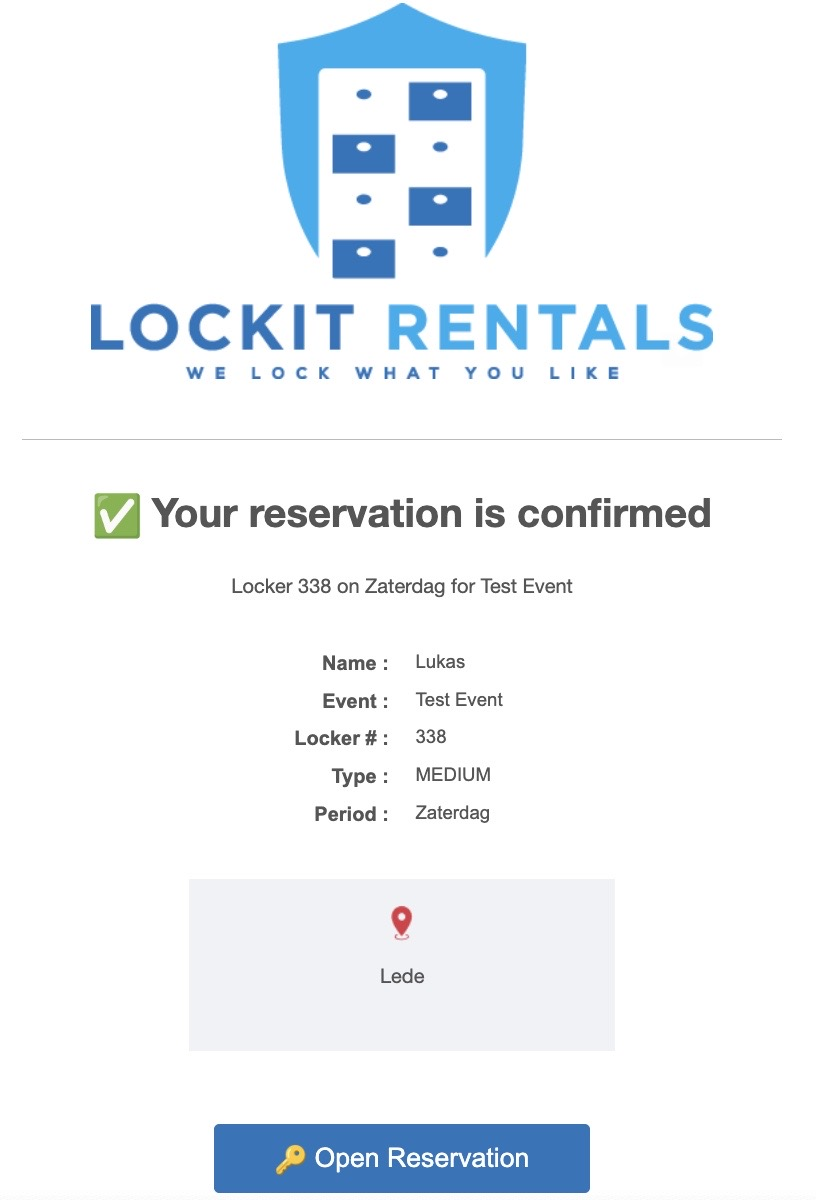
\includegraphics[width=0.5\textwidth]{graphics/F34_mailQR-code.jpg}
    \captionsetup{justification=centering, singlelinecheck=false}
    
    \caption{Een verstuurde mail afkostig van Lockit Rentals met in bijlage de teruggewonnen QR-code.}
    \label{fig:resultatEmailQR-code}
\end{figure}

\begin{figure}[h]
    \centering
    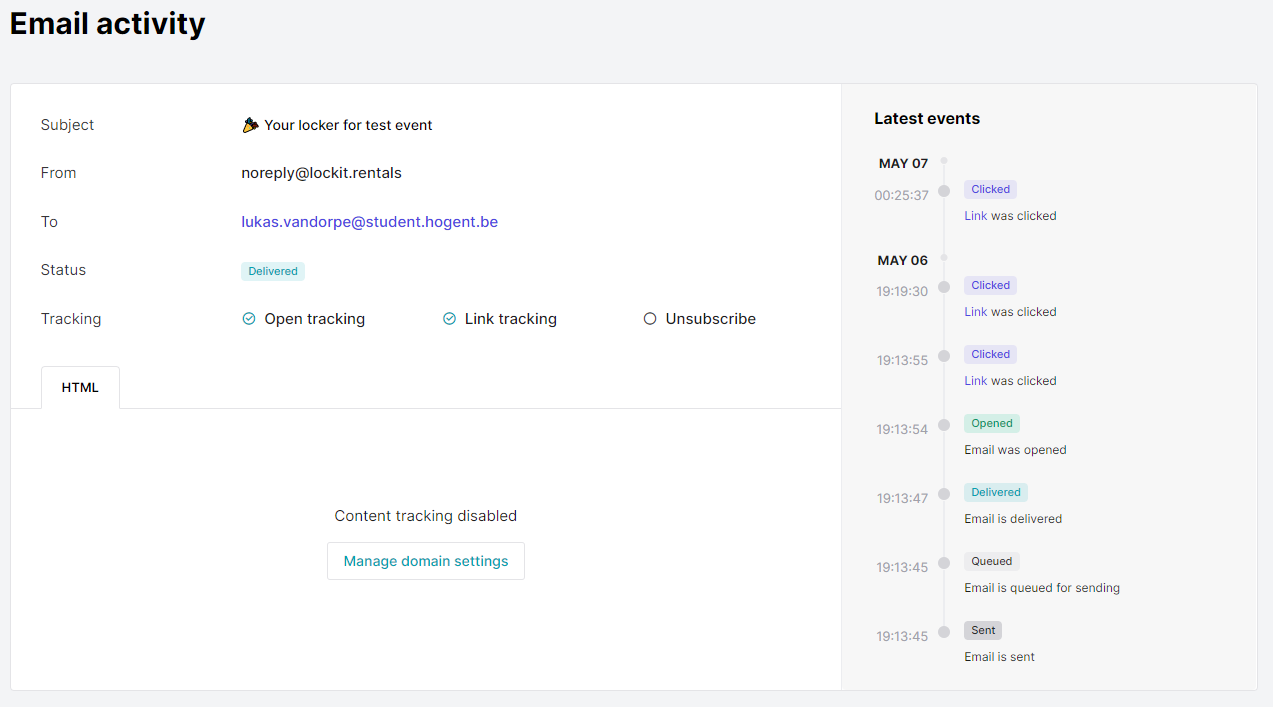
\includegraphics[width=0.8\textwidth]{graphics/F35_mailSender.png}
        \captionsetup{justification=centering,singlelinecheck=false}
    \caption{De tool 'Mail Sender' waarop we de verzonden mail kunnen traceren.}
    \label{fig:resultaatEmailSender}
\end{figure}











